\section{Two prescribed ports on one line}\label{c:same-side}
Fix two boundary ports at distance $l$ in a half-plane. The following
argument grows independent prefixes from them, then joins those prefixes
above their next common renewal level. The joining kernel must become
insensitive to a sublinear change of its endpoint separation. We prove
that regularity here, using the same pair process that controls the
length of the joining path.
The half-plane probability conclusion below is also established in
\cite[Proposition~5.8]{Renewal}. Here the common-level argument supplies
local regularity of the arch kernel as well as the length law, which we
then transfer to the same-side hexagon law.

\begin{theorem}[Same-side probability law]\label{c:same-side-law}
Under the critical half-plane law $w(\gamma)/K_l$, for every
$\varepsilon>0$,
\[
 \mathbb P\{l^{4/3-\varepsilon}\le L(\gamma)
                   \le l^{4/3+\varepsilon}\}\longrightarrow1.
\]
The same conclusion holds in the hexagons of Theorem~\ref{c:main} when both scaled
endpoints converge to distinct points in one side interior.
\end{theorem}
\subsection{Common blocks and lateral concentration}
We use the intersection-renewal construction discussed in
\cite[Section~1.1]{AlexanderBerger2016}, proving the required identities
directly. Distances along the base are physical distances, with port
spacing one; heights are in row units. Run two independent sequences of
upward irreducibles of law $p$, translating each new piece to the current
endpoint. Stop at their next common positive renewal height. Let $r$ be
the resulting mass on finite pairs of terminating sequences, initially
possibly a subprobability, and let $T$ be their common height.

A pair block contains one complete bridge segment from each sequence,
possibly made of several irreducibles. Let $D_*$ be the maximum of the
diameters of these two complete segments, and let $Y$ be the second
segment's lateral displacement minus the first's. In particular,
$|Y|\le2D_*$. Successive common blocks regenerate independently: testing
a prescribed pair of terminating sequences uses only the pieces up to
their termination.

\begin{lemma}[Common-block estimates]\label{c:pair-block-estimates}
The pair-block mass $r$ is a probability. For $x\ge1$,
\[
 r(T>x)+r(D_*>x)\le Cx^{-1/2}.
\]
If $Y^{(m)}$ is the sum of the lateral differences of $m$ independent
pair blocks, then
\[
 \sup_j\Pr(Y^{(m)}=j)\le Cm^{-2}\qquad(m\ge1).
\]
\end{lemma}
\begin{proof}
The common renewal masses are $B_h^2$, so
\[
 C(s)=\sum_{h\ge0}e^{-s h}B_h^2=(1-\hat r(s))^{-1}\asymp s^{-1/2},\qquad
 \hat r(s)=\sum r e^{-sT}.
\]
Sending $s$ to zero shows that $r$ has total mass one, and
$1-\hat r(s)\asymp s^{1/2}$ gives the height-tail estimate.
For the diameter estimate use \(s=D/x\) with \(D\) large fixed in \(C(s)\). The fraction containing a pair-block with \(D_*>x\) is at most \(C x^{-1/4}s^{-3/4}/C(s)<1/2\), using the diameter estimate on one total bridge and the ordinary \(B_h\) bound on the other. More explicitly put $d_s=1-\hat r(s)$ and $q_s=\mathbb E_r[e^{-sT};D_*>x]$. The fraction of terminated lists containing such a block is $q_s/(d_s+q_s)$, so the preceding bound below $1/2$ gives $q_s\le d_s=O(x^{-1/2})$; remove the discount below height \(x\), and above use the height tail from \(1-\hat r(s)\).



\paragraph{A lateral fluctuation in one common block.}
The common-height transform identifies the time scale. We next show that
the transverse difference fluctuates on the same scale; otherwise it
could not smooth a prescribed separation. We claim there are fixed \(D_1>D_0>0\) with
\[
 r(D_0 x\le |Y|\le D_1 x)\ge c x^{-1/2}
\]
for large \(x\). At every large height \(h\), the ordinary bridge kernel has mass \(\gtrsim h^{-1/4}\) of lateral displacements between two positive fixed multiples of \(h\). For clarity, using physical thickness \(d h\), go along the direction inclined at \(60^\circ\) to vertical to a pure tilted cut normal to that direction at distance near \((3/2)d h\) from the start, then vertically to the top, in small tolerances by the turned crossing estimate in Proposition~\ref{c:finite}(iii). The two legs lie on opposite sides of their joining cut. The first stays below the top, the second above the base, so they concatenate without mutual contacts and cross that cut exactly once. Average the concatenation indicator over a small fixed relative window of tilted levels. Its first moment is at least $ch^{-1/2}$. For two choices $t,t'$ in row units, splitting at both tilted cuts gives two outer crossings and the intervening difference bridge. Their joint cost is at most
\[
 Ch^{-1/2}(1+|t-t'|)^{-1/4}.
\]
The outer crossings are still paid by the two-cut upper estimate.
Averaging the gap factor over the order-$h$ window gives a second moment
of order at most $h^{-3/4}$. Cauchy--Schwarz therefore gives the asserted
mass of off-axis bridges.



Normalize \(C(1/x)\) to probability on terminated sequences. In heights \(x\le h\le 2x\), applying these displacement restrictions in opposite directions retains a positive probability of total absolute displacement difference at least \(a x\) for some \(a>0\). On the other hand the number of pair-blocks there (under the normalized sum over all heights) is geometric on \(0,1,\dots\), of mean \(O(x^{1/2})\), and the independent block laws conditional on that number are tilted by \(e^{-T/x}/\hat r(1/x)\). By \(|Y|\le2D_*\) the probability of any term with \(|Y|>D_1x\) is \(O(D_1^{-1/2})\), and the expectation of the absolute-value sum over terms with \(|Y|<D_0 x\) is \(O(\sqrt{D_0}\,x)\). Taking the window sufficiently wide, we must thus see a term within it with positive probability. The mean-count bound and tilt then imply the claim under \(r\).



\(Y\) has a symmetric law, on the integers since the endpoints have the same row stagger. Consequently \(Y^{(m)}\), the sum over \(m\) independent pair-blocks, has
\[
 \sup_j\Pr(Y^{(m)}=j)\le C m^{-2}.
\]
Indeed symmetrizing with an independent copy (bounded with positive probability), the window bound yields \(1-|\mathbb E e^{i\theta Y}|^2\gtrsim |\theta|^{1/2}\) near zero by taking \(x\) a sufficiently small fixed multiple of \(1/|\theta|\). Peaks repeat the modulus at zero and there are only finitely many on the torus since the support has at least two integers. Integrate the modulus to the \(m\)-th power.
\end{proof}

\subsection{Regularity of the joining kernel}
We next attach short prefixes and recover them from the completed arch.
Figure~\ref{c:pair-figure} shows this construction.

\begin{figure}[ht]
\centering
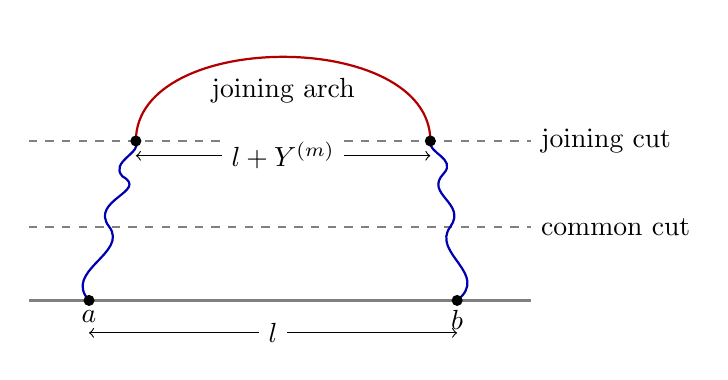
\begin{tikzpicture}[x=0.85cm,y=0.75cm,thick]
\draw[gray] (-0.3,0)--(7.2,0);
\draw[dashed,gray] (-0.3,1.25)--(7.2,1.25);
\draw[dashed,gray] (-0.3,2.7)--(7.2,2.7);
\draw[blue!70!black] (0.6,0) .. controls (0.2,0.5) and (1.2,0.8) .. (0.9,1.25)
 .. controls (0.6,1.7) and (1.5,1.85) .. (1.1,2.1)
 .. controls (0.9,2.35) and (1.4,2.5) .. (1.3,2.7);
\draw[blue!70!black] (6.1,0) .. controls (6.6,0.45) and (5.7,0.8) .. (6,1.25)
 .. controls (6.25,1.65) and (5.6,1.8) .. (5.9,2.15)
 .. controls (6.1,2.4) and (5.65,2.5) .. (5.7,2.7);
\draw[red!70!black] (1.3,2.7) .. controls (1.3,4.6) and (5.7,4.6) .. (5.7,2.7);
\fill (0.6,0) circle(2pt) node[below] {$a$};
\fill (6.1,0) circle(2pt) node[below] {$b$};
\fill (1.3,2.7) circle(2pt);
\fill (5.7,2.7) circle(2pt);
\node[right] at (7.2,1.25) {common cut};
\node[right] at (7.2,2.7) {joining cut};
\node at (3.5,3.55) {joining arch};
\draw[<->,thin] (0.6,-0.55)--(6.1,-0.55) node[midway,fill=white] {$l$};
\draw[<->,thin] (1.3,2.45)--(5.7,2.45) node[midway,fill=white] {$l+Y^{(m)}$};
\end{tikzpicture}
\caption{Two independent prefixes meet a common renewal height and are
joined above it. In the restricted small-prefix construction, the prefixes remain near their respective starting ports.
The first $m$ levels with exactly two crossings recover the sampled pair
blocks. This is a schematic: the lattice paths need not be monotone between
these marked levels.}\label{c:pair-figure}
\end{figure}

\begin{lemma}[Sublinear changes of the gap]\label{c:arch-kernel-regularity}
For positive integers $l,l'$ with $l\to\infty$ and $l'/l\to1$,
\[
 K_{l'}/K_l\longrightarrow1.
\]
\end{lemma}
\begin{proof}
For initial separation \(j\), call prefixes of \(m\) pair-blocks good if \(\sum_{i\le m}D_{*,i}<j/4\), of failure probability \(O(m/\sqrt j)\) by truncation. They are disjoint then, and we may join above the attained common level by any half-plane arch joining the endpoints. This gives
\[
 K_j\ge \mathbb E\,[{\bf1}_{\rm good} K_{j+Y^{(m)}}].
\]
Indeed product probabilities on the pair sequences are ordinary critical weights. The first \(m\) positive base-parallel levels having exactly two crossings of the output are precisely the \(m\) common renewals used: before reaching the joining level each branch must cross each level, and crossing just once is exactly renewal within that branch. The joining level itself has the two prescribed crossings. Thus the construction is injective.



\paragraph{Excluding a jump on a sublinear scale.}
Use monotonicity and the two-sided bounds of order \(l^{-5/4}\). If the conclusion failed, along a sequence there would be drops at least \(\epsilon l^{-5/4}\) between \(l-w\) and \(l+w\) with \(1\le w=o(l)\). For large integer scales \(q\) set \(m=\lfloor\sqrt q\rfloor\); then \(\Pr(Y^{(m)}\le -b q)\ge1/4\) with some small fixed \(b>0\), by Lemma~\ref{c:pair-block-estimates} and symmetry. Also \(\Pr(|Y^{(m)}|>Aq)=O(A^{-1/2})\) by the pair diameter tail and truncation. Fix \(A\) large. Choose \(w\ll q\ll l\) so the variation on \([l+ bq/4,l+(A+b+1)q]\) is \(o(l^{-5/4})\); arbitrarily many disjoint such bands at geometric scales are available between these two scales, and their variations sum to \(O(l^{-5/4})\). At \(j=l+\lfloor bq/2\rfloor\), on good prefixes with \(|Y^{(m)}|\le A q\) the arch factor on the right of the inequality is at least \(K_j-o(l^{-5/4})\). On those also having \(Y^{(m)}\le-bq\), the new gap lies below $l-w$, so the factor gains at least \(\epsilon l^{-5/4}\) over \(K_j\). Good has probability tending to one since $m/\sqrt j=O(\sqrt{q/l})$. The discarded tail loses at most $O(A^{-1/2})K_j$, whereas the gain occurs with probability at least $1/4-O(A^{-1/2})-o(1)$. Taking \(A\) sufficiently large in terms of \(\epsilon\) contradicts the construction inequality.
\end{proof}



\subsection{Concentration under the prescribed-gap law}
\begin{proof}[Proof of Theorem~\ref{c:same-side-law}]
Lemma~\ref{c:arch-kernel-regularity} shows that sublinear perturbations preserve the joining mass.
It remains to transfer the independent-prefix law and bound an unusually
long joining arch. Take \(m=\lfloor l^{1/2-\eta}\rfloor\) for small fixed \(\eta>0\). The good construction exhausts \(1-o(1)\) of total exact arch mass, since \(\sum D_{*,i}/l\to0\) in probability and the joining factor relative to \(K_l\) tends to 1 in probability there (and stays bounded on good prefixes). In the independent pair process the height after \(m\) grows as \(m^{2+o(1)}\) almost surely by the height transform and the power-sum argument of Proposition~\ref{c:renewal}. Each of the two individual cumulative lengths there grows as \((m^2)^{4/3+o(1)}\) by the almost sure individual irreducible-sequence laws, valid also along this subsequence of their renewals. Thus both prefixes' length exponents in \(l\) are arbitrarily close to \(4/3\) with probability tending to one by taking \(\eta\) small, which transfers to good constructed paths by bounded reweighting.



Finally bound the contribution among these paths with joining length above \(\tfrac12 l^{4/3+\epsilon}\). By the atom estimate and translating the first joining endpoint to a fixed origin it is at most
\[
 C m^{-2}\left(C R^{-1/4}+l^{-4/3-\epsilon} R^{13/12+o(1)}\right),\qquad R=l^{1+\gamma}.
\]
Indeed after summing over the other joining endpoint this uses the half-plane diameter bound above \(R\); for smaller diameters the summed length mass with this fixed start is bounded by translating to order \(R\) equivalent starts along the base of a common encompassing convex truncation of size \(O(R)\) and using the free-endpoints length bound \(R^{25/12+o(1)}\) by occupancy. Choose \(\gamma>0\) sufficiently small relative to \(\epsilon\) and then \(\eta>0\) sufficiently small that
\[
 2\eta<\gamma/4,\qquad 2\eta+13\gamma/12<\epsilon.
\]
Both displayed contributions are then $o(l^{-5/4})$. This proves the
half-plane length concentration.

For the hexagon, the prescribed same-side separation satisfies $l\asymp R$.
Proposition~\ref{c:connectors} gives normalizing mass at least
$cl^{-5/4}$ inside the hexagon. The absolute exceptional mass there is
at most the full half-plane exceptional mass, which is $o(l^{-5/4})$.
Dividing by the finite-domain normalizer transfers both length tails.

\end{proof}
